\documentclass[10pt]{article} % For LaTeX2e -- TMLR requires 10pt

% ---------------------------------------------------------------------------
% TMLR style file. For the arXiv/preprint version (de-anonymized), swap the
% line below for: \usepackage[preprint]{tmlr}
% For the accepted camera-ready version, use: \usepackage[accepted]{tmlr}
% ---------------------------------------------------------------------------
\usepackage{tmlr}

% tmlr.sty already loads xcolor, fancyhdr, and natbib -- do not re-load
% geometry (tmlr.sty sets its own page layout) or xcolor here.
\usepackage{amsmath,amssymb}
\usepackage{booktabs}
\usepackage{graphicx}
\usepackage{hyperref}
\usepackage{url}
\usepackage{caption}
\usepackage{enumitem}
\usepackage{amsthm}

\newtheorem{proposition}{Proposition}

\hypersetup{
  colorlinks=true,
  linkcolor=blue,
  citecolor=blue,
  urlcolor=blue,
}

\title{\bf Many Small Memories or Few Rich Memories?\\
\large A Matched-Budget Study of Memory Allocation in Small Language Models}

% TODO: fill in actual author name(s) and affiliation(s) before submitting.
\author{Author Name(s) \\ Affiliation}
\date{}

\begin{document}
\maketitle

\begin{abstract}
Language models that compress inference-time state can spend a fixed
persistent-memory budget in different ways. A model can store many
token-indexed states, as in a compressed KV cache, or compress context into
a smaller set of recurrent memory states. We study this allocation choice
under matched persistent-memory budgets, at context lengths up to
approximately 128 tokens -- a controlled memory-allocation study, not a
long-context evaluation. Across TinyStories and WikiText-103 language
modeling at 7M and 35M scale, compressed per-token memory gives lower
validation loss than a custom recurrent few-rich-memory model with the same
parameter count and persistent-memory budget. On synthetic exact-recall
tasks, per-token memory is the most reliable strategy tested: it solves
dense copy and needle retrieval across repeated runs, and it beats an RMT-style
memory-token baseline in direct synthetic comparisons. At the same time,
RMT-style memory tokens are much stronger than the custom recurrent
baseline on long-gap single-fact needle retrieval, showing that few-rich
memory is not uniformly weak and that the recurrence mechanism matters. We
formalize the update rules of each mechanism, and provide a set of
diagnostic analyses -- including a slot-allocation shape sweep, a
norm-boundedness argument that localizes a known write-scale instability,
a token-salience retention study, and multiple independent training runs
for the highest-impact comparisons -- that together support the following
claim: under matched budgets, per-token memory is the strongest strategy
tested for exact-recall tasks and language modeling, while few-rich
recurrent memory can be effective for sparse salient retrieval when the
update mechanism is well matched to the task.
\end{abstract}

% ===========================================================================
\section{Introduction}
% ===========================================================================

Memory is one of the central bottlenecks in language modeling at any
context length beyond the trivial. A standard Transformer stores a key and
value for every previous token in every layer. This is accurate but
expensive: the memory grows linearly with sequence length, layer count,
and hidden size. A common response is to compress memory. However,
compression is not one design choice. The same persistent-memory budget
can be allocated across many small token-indexed states or concentrated
into a fixed set of richer recurrent states. We study this trade-off in a
controlled, small-scale setting -- at context lengths up to approximately
128 tokens -- rather than as a long-context capability claim.

This paper asks a deliberately narrow question:

\begin{quote}
\itshape
Given the same persistent inference-time memory budget, is it better to keep
many small token-indexed memories, or fewer rich recurrent memories?
\end{quote}

We study this question in a small but controlled setting. The main
comparison is between compressed per-token KV memory and recurrent memory
under matched persistent-memory floats. We also include a baseline
Transformer with full KV memory, structured associative recurrent variants,
and an RMT-style memory-token baseline adapted from the public Recurrent
Memory Transformer design \citep{bulatov2022rmt}.

The answer is not a simple ``recurrent memory is bad.'' Per-token memory is
the strongest strategy tested for language modeling and exact synthetic
recall, but RMT-style memory tokens substantially improve long-gap
single-fact retrieval over the custom recurrent updater. The resulting
picture is task-dependent: dense exact recall favors many token-indexed
states, while sparse salient recall can benefit from recurrent memory
tokens.

\paragraph{Contributions.}
\begin{itemize}[leftmargin=*]
  \item A controlled, matched-budget comparison of memory allocation shape
  (many-small vs.\ few-rich) that is explicitly separated from update
  mechanism (naive pooling vs.\ structured associative read/write vs.\
  RMT-style memory tokens), with formal update rules for each (Section~\ref{sec:models}).
  \item A methodological framing that separates \emph{learned parameters}
  from \emph{persistent per-sequence memory}, applied consistently across
  every architecture compared (Section~\ref{sec:memory-budget}).
  \item An honest negative result on structured associative addressing,
  and a positive but bounded result on RMT-style memory tokens, both
  confirmed across three independent training runs
  (Section~\ref{sec:results}, Appendix~A).
\end{itemize}

% ===========================================================================
\section{Related Work}
\label{sec:related-work}
% ===========================================================================

\paragraph{Segment recurrence and compressed context.}
Transformer-XL \citep{dai2019transformerxl} caches hidden states across
segments to extend effective context through segment-level recurrence.
Compressive Transformer \citep{rae2020compressive} extends this idea by
compressing older activations into a smaller memory rather than discarding
them. Block-Recurrent Transformers \citep{hutchins2022blockrecurrent}
maintain recurrent state vectors across blocks and update them jointly with
the current token block. These approaches establish recurrence and
compression as practical alternatives to retaining the full history, but
they do not directly isolate the question studied here: under a fixed
persistent memory budget, how should that capacity be distributed across
memory items?

\paragraph{Recurrent memory tokens and learned long-term memory.}
Recurrent Memory Transformer (RMT) \citep{bulatov2022rmt} introduces
learned memory tokens that are carried between segments and updated through
the Transformer's own self-attention. Associative Recurrent Memory
Transformer (ARMT) \citep{rodkin2024armt} extends this framework with
associative memory, while TransformerFAM \citep{hwang2024transformerfam}
introduces a feedback-attention mechanism for recurrent working memory.

Other work moves further toward learned persistent state. LongMem
\citep{wang2023longmem} augments a language model with an external
long-term memory and retrieval mechanism. Titans \citep{behrouz2025titans}
combines attention-based short-term memory with a learned neural memory
that is updated during inference. These systems motivate the broader
few-rich design space, where historical information is compressed into a
limited number of persistent states rather than retained explicitly for
every token.

Our RMT-style baseline follows the core RMT memory-token mechanism. Our
associative recurrent variant is an independent small-scale implementation
of explicit read/write addressing inspired by associative-memory
approaches; it is not a reproduction of ARMT, and our results should not be
interpreted as a claim about ARMT's reported performance.

\paragraph{KV-cache compression and reduced per-token state.}
A complementary family of methods preserves token-indexed memory while
reducing the amount of state stored per token. Grouped-Query Attention
(GQA) \citep{ainslie2023gqa} reduces KV-cache size by sharing key/value
heads across multiple query heads. Multi-head Latent Attention (MLA)
\citep{deepseek2024v2} instead represents per-token key/value information
through a lower-dimensional learned latent representation. Dynamic Memory
Compression (DMC) \citep{nawrot2024dmc} learns how KV states should be
merged or compressed online, with compression behavior varying across
heads and layers.

These methods are conceptually close to our many-small condition: token
identity remains explicitly represented, but fewer dimensions or states
are allocated to each token. Our goal is not to introduce another
KV-compression mechanism, but to compare this allocation strategy directly
against storing the same total persistent-memory capacity in a smaller
number of richer recurrent states.

Other approaches reduce memory consumption without changing the number of
stored token positions. KIVI \citep{liu2024kivi}, for example, applies
low-bit quantization to cached keys and values. Quantization is orthogonal
to the allocation problem considered here and could in principle be
applied to either many-small or few-rich memory.

\paragraph{KV eviction, selection, and non-uniform allocation.}
Another line of work reduces memory by retaining only selected historical
tokens. H$_2$O \citep{zhang2023h2o} identifies heavy-hitter tokens based on
their accumulated attention importance. Scissorhands
\citep{liu2023scissorhands} exploits persistence in token importance to
maintain a bounded cache, while SnapKV \citep{li2024snapkv} identifies
important prompt positions using attention patterns before generation.
PyramidKV \citep{cai2025pyramidkv} further considers non-uniform allocation
across Transformer layers.

Query-dependent approaches adapt the retained memory to the current
computation. Quest \citep{tang2024quest} performs query-aware selection of
KV pages, while DuoAttention \citep{xiao2025duoattention} distinguishes
retrieval heads, which require access to long-range KV states, from
streaming heads that can operate with a bounded recent cache. Together,
these works show that inference memory need not be allocated uniformly
across tokens, layers, or attention heads.

Our study investigates a different axis. Rather than asking \emph{which}
token-indexed states should be retained, we ask whether a matched memory
budget should remain distributed across many token-indexed states at all,
or instead be concentrated into fewer recurrent states.

\paragraph{Retrieval memories, compressed summaries, and hybrid designs.}
Memorizing Transformers \citep{wu2022memorizing} retrieve from a large
external store of historical key--value pairs rather than compressing
history into a small recurrent state. Infini-attention
\citep{munkhdalai2024infini} combines local attention with a continuously
updated compressive memory. MELODI \citep{chen2024melodi} represents
context through hierarchical short-term and long-term memories and
explicitly analyzes memory capacity, making it closely related to the
resource-oriented view adopted here.

Key-Value Means (KVM) \citep{goldstein2026kvm} introduces expandable
block-recurrent compressed memory that can interpolate between a compact
recurrent state and a growing KV-like representation. KVM is particularly
close in spirit to our many-small/few-rich framing because it exposes a
continuum between these extremes. Our study takes a complementary
approach: rather than proposing a mechanism that moves along this
continuum, we attempt to isolate allocation geometry itself as the
experimental variable.

\paragraph{Constant-state and recurrent alternatives to attention.}
Several architectures avoid a growing KV cache by replacing global
attention with recurrent or state-space computation. Mamba
\citep{gu2023mamba} uses a selective state-space recurrence whose inference
state does not grow with sequence length. RetNet \citep{sun2023retnet}
supports parallel, recurrent, and chunkwise-recurrent formulations of its
retention operator. RWKV \citep{peng2023rwkv} similarly combines
Transformer-like parallel training with RNN-like recurrent inference,
while Griffin \citep{de2024griffin} combines gated linear recurrence with
local attention.

These systems naturally occupy the few-rich side of our conceptual
spectrum, but direct comparisons would change both the memory geometry and
the underlying sequence-modeling operator. We therefore discuss them as
broader context rather than treating them as matched baselines.

StreamingLLM \citep{xiao2023streaming} occupies a different point in the
design space: it retains a bounded sliding window together with a small
number of attention-sink tokens. Its persistent state is bounded but
remains explicitly token-indexed, illustrating that fixed-memory inference
does not necessarily require recurrent summarization.

\paragraph{How this paper differs.}
Most work above proposes a single new mechanism and compares it against a
generic baseline. We instead hold the persistent-memory budget exactly
fixed and independently vary both the allocation shape (many-small vs.\
few-rich, and the slot-count/dimension split within few-rich) and the
update mechanism (pooling vs.\ associative read/write vs.\ RMT-style memory
tokens) inside one shared codebase, reporting parameters and memory floats
separately throughout.

% ===========================================================================
\section{Memory-Budget Framing}
\label{sec:memory-budget}
% ===========================================================================

We report two quantities separately for every model:

\begin{itemize}[leftmargin=*]
  \item \textbf{Parameters:} learned weights shared across examples.
  \item \textbf{Persistent memory floats:} per-sequence inference-time state
  carried forward to represent prior context.
\end{itemize}

This distinction matters. Learned memory tokens or read/write projections
are parameters. KV states, compressed token memories, and recurrent states
that must be carried for each active sequence are persistent memory. A
fixed learned initial state (e.g., a learned initial memory value) is a
parameter, not persistent memory, since it does not grow or change with the
input sequence on its own.

For a standard KV cache, the persistent memory is
\begin{equation}
  M_{\text{baseline}} = L \times 2 \times L_{\text{seq}} \times d_{\text{model}},
\end{equation}
where $L$ is the number of layers, $L_{\text{seq}}$ is sequence length,
$d_{\text{model}}$ is hidden size, and the factor of two counts keys and
values. For compressed per-token memory, the hidden state remains wide but
each token stores compressed keys and values of dimension $d_{\text{mem}}$:
\begin{equation}
  M_{\text{per-token}} = L \times 2 \times L_{\text{seq}} \times d_{\text{mem}}.
\end{equation}
For recurrent memory (custom recurrent, associative, and RMT-style), the
persistent state is a fixed table of $n$ memory slots of dimension
$d_{\text{r}}$, independent of $L_{\text{seq}}$:
\begin{equation}
  M_{\text{recurrent}} = n \times d_{\text{r}}.
\end{equation}
Note the structural difference: $M_{\text{per-token}}$ grows with
$L_{\text{seq}}$, while $M_{\text{recurrent}}$ does not. This is the
allocation trade-off under study, not an incidental implementation detail --
matching budgets across model types therefore means matching $M$ at a
\emph{specific} $L_{\text{seq}}$, and the comparison is only well posed at
that fixed length.

% ===========================================================================
\section{Models}
\label{sec:models}
% ===========================================================================

\begin{figure}[h]
\centering
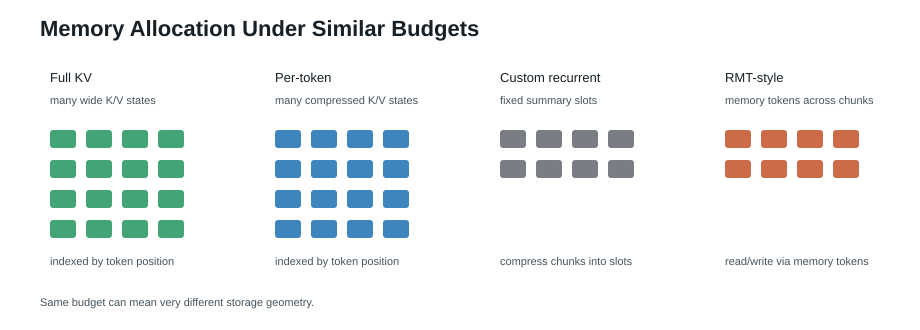
\includegraphics[width=0.95\linewidth]{figures/memory_layout.pdf}
\caption{Persistent-memory allocation shape across the four architectures
compared, at equal total memory-float budget: full KV cache, per-token
compressed memory (many-small), custom recurrent memory (few-rich), and
RMT-style memory tokens. The same budget produces very different storage
shapes depending on how it is allocated.}
\label{fig:memory_layout}
\end{figure}

Figure~\ref{fig:memory_layout} illustrates the four allocation shapes
compared throughout this paper before we define each model formally.

\subsection{Baseline Transformer}
The baseline is a decoder-only Transformer with RMSNorm, RoPE, SwiGLU MLPs,
causal self-attention, and tied embeddings. It uses the full KV cache and
therefore has the largest persistent-memory budget in the main tables.

\subsection{Per-Token Compressed Memory}
The per-token model keeps memory indexed by token position, but compresses
the key/value path to dimension $d_{\text{mem}} < d_{\text{model}}$. Each
token stores a smaller key and value per layer. Attention is performed in
compressed memory space and projected back to the model hidden size. This
is the ``many-small'' strategy: its persistent memory budget grows with
sequence length, but each unit of that budget is addressed directly to a
specific token.

\subsection{Custom Recurrent Memory}
\label{sec:custom-recurrent}
The custom recurrent model processes text in chunks of size $c$ and carries
a fixed memory table $\mathbf{m}_t \in \mathbb{R}^{n \times d_r}$ between
chunks $t$. After chunk $t$, token outputs $\mathbf{h}_t \in
\mathbb{R}^{c \times d_{\text{model}}}$ are summarized via one of three
update styles -- mean pooling, cross-attention, or a last-token update -- to
produce a candidate $\mathbf{\tilde m}_t$, and the memory is updated through
a gated combination:
\begin{equation}
  \mathbf{m}_{t+1} = (1 - \mathbf{g}_t) \odot \mathbf{m}_t + \mathbf{g}_t \odot \mathbf{\tilde m}_t,
  \qquad \mathbf{g}_t = \sigma\!\big(W_g [\mathbf{m}_t ; \mathbf{\tilde m}_t]\big),
  \label{eq:gate}
\end{equation}
with $\odot$ elementwise multiplication and $\sigma$ the sigmoid function.
This is the initial ``few-rich'' strategy: a fixed number of slots
regardless of sequence length.

\subsection{Associative Recurrent Memory}
\label{sec:assoc-model}
The associative variant replaces the pooled candidate $\mathbf{\tilde
m}_t$ in Equation~\ref{eq:gate} with an explicit content-addressed write.
Fixed learned write queries $Q_w \in \mathbb{R}^{n \times d_r}$ attend over
token keys $K_t = W_k \mathbf{h}_t$ to produce
\begin{equation}
  \mathbf{\tilde m}_t = \operatorname{softmax}\!\left(\frac{Q_w K_t^\top}{\sqrt{d_r}}\right) V_t,
  \qquad V_t = W_v \mathbf{h}_t,
\end{equation}
and reads are symmetric: token queries attend over fixed learned read keys
$K_r \in \mathbb{R}^{n \times d_r}$ to retrieve from the current memory
values. Only $\mathbf{m}_t$ (the memory \emph{values}) is per-sequence
state; $Q_w$, $K_r$, and the projections $W_k, W_v$ are parameters, fixed
across the sequence.

Because Equation~\ref{eq:gate} is an elementwise convex combination of
$\mathbf{m}_t$ and $\mathbf{\tilde m}_t$, its magnitude cannot grow beyond
what is fed into it:

\begin{proposition}
For any elementwise gate $\mathbf{g}_t \in [0,1]^{d}$, the update
$\mathbf{m}_{t+1} = (1-\mathbf{g}_t)\odot \mathbf{m}_t + \mathbf{g}_t \odot
\mathbf{\tilde m}_t$ satisfies, per coordinate $i$,
$|m_{t+1,i}| \le \max(|m_{t,i}|, |\tilde m_{t,i}|)$, and hence
$\|\mathbf{m}_{t+1}\|_\infty \le \max(\|\mathbf{m}_t\|_\infty,
\|\mathbf{\tilde m}_t\|_\infty)$.
\end{proposition}
\begin{proof}
For each coordinate $i$, $m_{t+1,i}$ is a convex combination of $m_{t,i}$
and $\tilde m_{t,i}$ with weight $g_{t,i} \in [0,1]$, so $m_{t+1,i}$ lies on
the segment between the two values and cannot exceed the larger of their
magnitudes. Taking the maximum over coordinates gives the $\ell_\infty$
bound.
\end{proof}

Proposition~1 also provides a diagnostic principle: any anomalous growth
in memory magnitude must originate in the candidate representation
$\mathbf{\tilde m}_t$ -- specifically in the write projection $W_v$ or
upstream token representations -- rather than in the gated update
itself. We exploit this to motivate write-source normalization as a
targeted stabilization mechanism, rather than clipping memory states
directly. As reported in Section~\ref{sec:assoc-negative} and Appendix~A,
this combination of explicit read/write addressing and write-source
normalization does not produce consistent retrieval improvements across
the settings we evaluate.

\subsection{RMT-Style Memory Tokens}
The RMT-style baseline wraps each chunk with $n$ memory tokens, adapted
from the public Recurrent Memory Transformer design
\citep{bulatov2022rmt}. Writing $\mathbf{m}_t$ for the incoming memory
state and $\mathbf{x}_t$ for the chunk's token embeddings, the model
processes the concatenation $[\mathbf{m}_t ; \mathbf{x}_t ; \mathbf{m}_t]$
(memory as both prefix and suffix) through the local Transformer layers
under a causal mask $\mathcal{C}$ satisfying
\begin{equation}
  \mathcal{C}(i,j) = \begin{cases}
    1 & \text{if } j \le i \text{ and } j \notin \text{suffix positions}, \\
    0 & \text{otherwise,}
  \end{cases}
\end{equation}
so that no predicted token can attend to the write-side (suffix) memory,
preserving causality. The output at the suffix positions becomes
$\mathbf{m}_{t+1}$. The learned initial memory value $\mathbf{m}_0$ is a
parameter (Section~\ref{sec:memory-budget}); $\mathbf{m}_t$ for $t>0$ is persistent memory. This
published-style recurrent mechanism is much stronger than the custom
recurrent updater on long-gap needle retrieval, but it does not beat
per-token memory in direct synthetic comparisons.

% ===========================================================================
\section{Experimental Setup}
% ===========================================================================

\subsection{Real-Data Language Modeling}
We train on TinyStories \citep{eldan2023tinystories} and WikiText-103
\citep{merity2017wikitext} using a GPT-2 \texttt{tiktoken} tokenizer. Each
model sees one full pass over the training tokens. Validation is run in
full at the final evaluation step. We report validation loss, perplexity,
tokens/sec, peak VRAM, parameter count, and persistent memory floats. The
repository contains both 7M-scale and 35M-scale runs; the 35M tables are
the main real-data evidence.

\subsection{Synthetic Recall}
\label{sec:synthetic-recall}
We define three synthetic tasks over a vocabulary $\mathcal{V}$. Let
$U(\mathcal{V})$ denote uniform sampling.

\paragraph{Copy.} A sequence $\mathbf{s} = (s_1, \dots, s_k)$, $s_i \sim
U(\mathcal{V})$, is followed by a delimiter token, after which the target
is $\mathbf{s}$ itself. Accuracy is the fraction of the $k$ target
positions where the model's predicted token matches $\mathbf{s}$ exactly.
This tests dense exact recall of $k$ simultaneous token identities.

\paragraph{Needle.} A single value $v \sim U(\mathcal{V})$ is placed at a
fixed position, followed by $g$ filler tokens (the ``gap''), followed by a
query whose target is $v$. Accuracy is $\mathbf{1}[\hat v = v]$ averaged
over examples. This tests sparse single-fact retrieval as a function of
gap length $g$.

\paragraph{Random KV.} $p$ key--value pairs $(k_i, v_i)$, $k_i, v_i \sim
U(\mathcal{V})$ with distinct keys, are presented, followed by a query key
$k_j$ whose target is $v_j$. Accuracy is $\mathbf{1}[\hat v = v_j]$
averaged over examples and query positions. This tests multi-pair
associative recall as a function of the number of stored pairs $p$.

Synthetic recall is measured as teacher-forced next-token accuracy at the
relevant target positions, not free-form autoregressive generation. This
isolates whether the correct information is accessible in memory at the
point of use, independent of the model's ability to generate a full
correct continuation autoregressively. Every synthetic accuracy number in
this paper, including the token-salience and retention analysis in
Section~\ref{sec:salience-retention}, should be read under this scope: as a
measure of what is accessible in memory, not as a measure of end-to-end
free-generation robustness.

Synthetic RMT-vs-per-token and RMT-vs-custom-recurrent comparisons are run
across three independent runs for the highest-impact cells (the settings
where an initial single run showed the largest or most surprising effect).

% ===========================================================================
\section{Results}
\label{sec:results}
% ===========================================================================

\subsection{Real-Data Language Modeling}
\label{sec:realdata-results}
TinyStories and WikiText-103 under the matched compressed-memory budget
(Table~\ref{tab:realdata}). The original 35M recurrent shape used 8 very
wide slots (\texttt{8x32768}). A fairer many-slot shape
(\texttt{128x2048}) improves recurrent loss slightly on both datasets, but
does not close the gap to per-token memory. This reduces the concern that
the main recurrent result is only a bad slot-shape artifact.

The two training runs of the \texttt{128x2048} recurrent model on
WikiText-103 show substantially higher variance than any other configuration
in this table (3.7861 and 3.7130, a gap of 0.073). This variance is
shape-specific rather than a general property of WikiText-103 or recurrent
architectures: the \texttt{8x32768} recurrent shape on the same dataset
shows ordinary run-to-run variation (0.0061, consistent with baseline and
per-token), and every other multi-run configuration falls in the 0.0007--0.0066
range. We report the mean and standard deviation for this configuration
and flag the width of this interval explicitly; the \texttt{8x32768} shape,
which shows stable runs, is the primary recurrent evidence in this table.

This choice of a many-slot, narrow-dimension shape is itself supported by a
finer-grained sweep at synthetic scale, holding the total budget fixed at
32,768 floats (Table~\ref{tab:shapesweep}). Many-slot shapes
(\texttt{64x512}) matched or slightly outperformed few-slot, wide-dimension
shapes (\texttt{8x4096}) at copy length 32, and were comparable at length
64 -- across every shape tested, none closes the gap to per-token memory's
near-ceiling performance on the same task, so the shape sweep supports the
allocation claim rather than complicating it.

\begin{table}[h]
\centering
\caption{Recurrent shape sweep, copy task, fixed 32,768-float budget.}
\label{tab:shapesweep}
\begin{tabular}{lrrr}
\toprule
Shape & Copy-16 & Copy-32 & Copy-64 \\
\midrule
\texttt{8x4096}  & 0.942 & 0.045 & 0.030 \\
\texttt{16x2048} & 0.942 & 0.057 & 0.031 \\
\texttt{32x1024} & 0.942 & 0.046 & 0.030 \\
\texttt{64x512}  & 0.942 & 0.069 & 0.031 \\
\bottomrule
\end{tabular}
\end{table}

\begin{table}[h]
\centering
\caption{Real-data language modeling at 35M scale. Params and Mem Floats
are reported separately per the accounting in Section~\ref{sec:memory-budget}.
Val.\ loss is reported as mean $\pm$ std across two independent training
runs where both are available; unmarked values are from a single run.}
\label{tab:realdata}
\begin{tabular}{llrrrr}
\toprule
Dataset & Model & Val Loss & Perplexity & Params & Mem Floats \\
\midrule
TinyStories  & Baseline                     & $1.547 \pm 0.005$ & 4.70  & 38{,}179{,}584 & 786{,}432 \\
TinyStories  & Per-token                    & $1.581 \pm 0.001$ & 4.86  & 35{,}431{,}680 & 262{,}144 \\
TinyStories  & Recurrent \texttt{8x32768}   & $1.709 \pm 0.003$   & 5.52  & 35{,}431{,}680 & 262{,}144 \\
TinyStories  & Recurrent \texttt{128x2048}  & $1.703 \pm 0.0004$ & 5.49  & 35{,}450{,}112 & 262{,}144 \\
\addlinespace
WikiText-103 & Baseline                     & $3.621 \pm 0.001$  & 37.38 & 38{,}179{,}584 & 786{,}432 \\
WikiText-103 & Per-token                    & $3.686 \pm 0.004$  & 39.88 & 35{,}431{,}680 & 262{,}144 \\
WikiText-103 & Recurrent \texttt{8x32768}   & $3.794 \pm 0.004$   & 44.44 & 35{,}431{,}680 & 262{,}144 \\
WikiText-103 & Recurrent \texttt{128x2048}  & $3.750 \pm 0.052$  & 42.50 & 35{,}450{,}112 & 262{,}144 \\
\bottomrule
\end{tabular}
\end{table}

At 7M scale, the same ordering holds, and the smaller scale additionally lets
us compare two recurrent update styles directly under an identical budget
(Table~\ref{tab:realdata7m}): mean-GRU and cross-attention pooling perform
similarly to each other, and both trail per-token by a comparable margin to
what is observed at 35M.

\begin{table}[h]
\centering
\caption{Real-data language modeling at 7M scale.}
\label{tab:realdata7m}
\begin{tabular}{llrrrr}
\toprule
Dataset & Model & Val Loss & Perplexity & Params & Mem Floats \\
\midrule
TinyStories  & Baseline                        & 2.0459 & 7.74 & 6{,}957{,}824 & 65{,}536 \\
TinyStories  & Per-token                       & 2.0850 & 8.04 & 6{,}942{,}976 & 32{,}768 \\
TinyStories  & Recurrent, mean-GRU              & 2.1771 & 8.82 & 6{,}942{,}464 & 32{,}768 \\
TinyStories  & Recurrent, cross-attn            & 2.1788 & 8.84 & 6{,}942{,}976 & 32{,}768 \\
\addlinespace
WikiText-103 & Baseline                        & 4.3454 & 77.12 & 6{,}957{,}824 & 65{,}536 \\
WikiText-103 & Per-token                       & 4.3592 & 78.19 & 6{,}942{,}976 & 32{,}768 \\
WikiText-103 & Recurrent, cross-attn            & 4.4231 & 83.36 & 6{,}942{,}976 & 32{,}768 \\
\bottomrule
\end{tabular}
\end{table}

\begin{figure}[h]
\centering
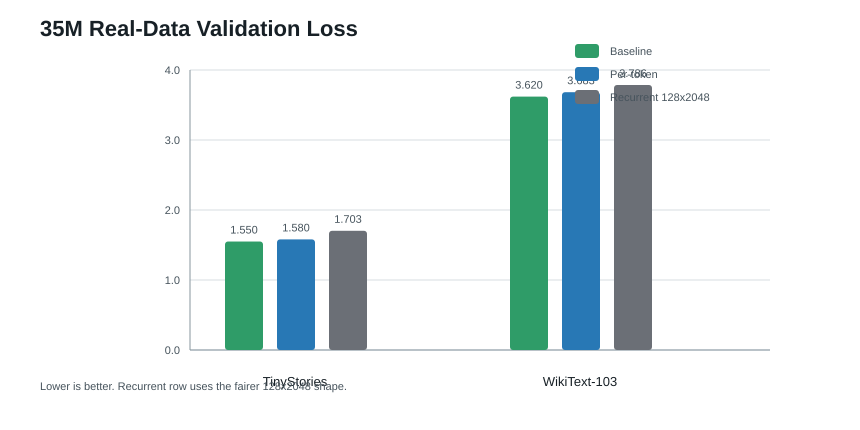
\includegraphics[width=0.85\linewidth]{figures/real_lm_loss.pdf}
\caption{Validation loss at 35M scale, TinyStories and WikiText-103, for
all four real-data configurations in Table~\ref{tab:realdata}. Per-token
memory beats both recurrent shapes on both datasets at matched
persistent-memory budget.}
\label{fig:real_lm_loss}
\end{figure}

\subsection{Synthetic Exact Recall Across Length}
\label{sec:base-synthetic}
\label{sec:longcontext}

We test copy and needle recall across the full length range studied in
this paper, from length/gap 8 up to copy length 512 and needle gap 1024,
across all four architectures. Two budget designs are combined here:
lengths 8--64 match recurrent memory's budget to per-token's own budget
at each length individually (growing from 4{,}864 floats at length 8 to
33{,}536 at length 64); lengths 128 and above fix recurrent memory at a
constant 32,768 floats (matching the shape-sweep design in
Table~\ref{tab:shapesweep}). RMT-style memory is evaluated at copy lengths
16, 32, 64, 128, and 256, and needle gaps 16, 32, 64, and 128. The 32/64
RMT rows are three-run means from Table~\ref{tab:pertoken_vs_rmt}; longer
RMT rows are single runs. RMT copy length 512 and needle gaps beyond 128
remain incomplete, since earlier attempts ran out of GPU memory.

\begin{table}[h]
\centering
\caption{Copy accuracy across length. RMT-style at 32/64 is the
three-run mean from Table~\ref{tab:pertoken_vs_rmt}; RMT-style at 16, 128,
and 256 is from single runs. ``--'' marks cells not yet run.}
\label{tab:basecopy}
\begin{tabular}{lrrrr}
\toprule
Copy Length & Baseline & Per-token & Recurrent & RMT-style \\
\midrule
8   & 1.000 & 1.000 & 1.000 & -- \\
16  & 1.000 & 1.000 & 0.942 & 0.922 \\
32  & 1.000 & 1.000 & 0.045 & 0.680 \\
64  & 1.000 & 1.000 & 0.030 & 0.031 \\
128 & 1.000 & 1.000 & 0.023 & 0.023 \\
256 & 0.996 & 0.996 & 0.019 & 0.018 \\
512 & 0.998 & 1.000 & 0.016 & -- \\
\bottomrule
\end{tabular}
\end{table}

\begin{table}[h]
\centering
\caption{Needle accuracy across gap. RMT-style at 32/64 is the
three-run mean from Table~\ref{tab:pertoken_vs_rmt}; RMT-style at 16 and
128 is from single runs. ``--'' marks cells not yet run.}
\label{tab:baseneedle}
\begin{tabular}{lrrrr}
\toprule
Gap Length & Baseline & Per-token & Recurrent & RMT-style \\
\midrule
8    & 1.000 & 1.000 & 1.000 & -- \\
16   & 1.000 & 1.000 & 1.000 & 1.000 \\
32   & 1.000 & 1.000 & 0.016 & 0.702 \\
64   & 1.000 & 1.000 & 0.015 & 0.877 \\
128  & 1.000 & 1.000 & 0.015 & 0.807 \\
256  & 1.000 & 1.000 & 0.014 & -- \\
512  & 1.000 & 1.000 & 0.015 & -- \\
1024 & 1.000 & 1.000 & 0.018 & -- \\
\bottomrule
\end{tabular}
\end{table}

Baseline and per-token memory solve both tasks almost perfectly across
the entire range, length 8 through 512--1024. Custom recurrent memory
holds up through length/gap 16, collapses sharply between 16 and 32, and
never recovers -- not at length 64 under a per-token-matched budget, and
not at length 512 or gap 1024 under a fixed 32,768-float budget, 8--16x
beyond the original length-64 evidence. RMT-style memory is markedly
stronger than custom recurrent on needle wherever it has been tested
(0.702--0.877 vs.\ 0.015--0.016 at gaps 32--128), but the picture is
incomplete beyond gap 128. On copy, RMT-style memory matches custom
recurrent near chance at lengths 128 and 256, so it does not currently
change the dense-copy conclusion. Completing the RMT-style rows at copy
length 512 and needle gaps 256, 512, and 1024 is the direct next step for
this section; the most consequential open cell is needle-256, which would
show whether RMT-style memory's advantage over custom recurrent
(Section~\ref{sec:rmt-recurrent-story}) persists past gap 128 or
plateaus.



Per-token memory is the strongest exact-recall model tested. In direct
comparison with RMT-style memory, it solves copy and needle across all
tested runs, and it also wins random KV retrieval
(Table~\ref{tab:pertoken_vs_rmt}). The KV-16 separation is stronger than an
average-only comparison would suggest: RMT's highest observed value
(0.159) remains below per-token's lowest (0.163).

\begin{table}[h]
\centering
\caption{Per-token vs.\ RMT-style memory, synthetic tasks, three independent training runs.}
\label{tab:pertoken_vs_rmt}
\begin{tabular}{llrrrrr}
\toprule
Task & Model & Run 1 & Run 2 & Run 3 & Mean & Std \\
\midrule
Copy-32       & Per-token & 1.000 & 1.000 & 1.000 & 1.000 & 0.000 \\
Copy-32       & RMT-style & 0.112 & 0.963 & 0.964 & 0.680 & 0.491 \\
Copy-64       & Per-token & 1.000 & 1.000 & 1.000 & 1.000 & 0.000 \\
Copy-64       & RMT-style & 0.031 & 0.030 & 0.031 & 0.031 & 0.000 \\
Needle-32     & Per-token & 1.000 & 1.000 & 1.000 & 1.000 & 0.000 \\
Needle-32     & RMT-style & 0.938 & 0.677 & 0.491 & 0.702 & 0.225 \\
Needle-64     & Per-token & 1.000 & 1.000 & 1.000 & 1.000 & 0.000 \\
Needle-64     & RMT-style & 0.903 & 0.966 & 0.763 & 0.877 & 0.104 \\
Random KV-16  & Per-token & 0.163 & 0.167 & 0.173 & 0.168 & 0.005 \\
Random KV-16  & RMT-style & 0.067 & 0.159 & 0.067 & 0.098 & 0.053 \\
\bottomrule
\end{tabular}
\end{table}

\begin{figure}[h]
\centering
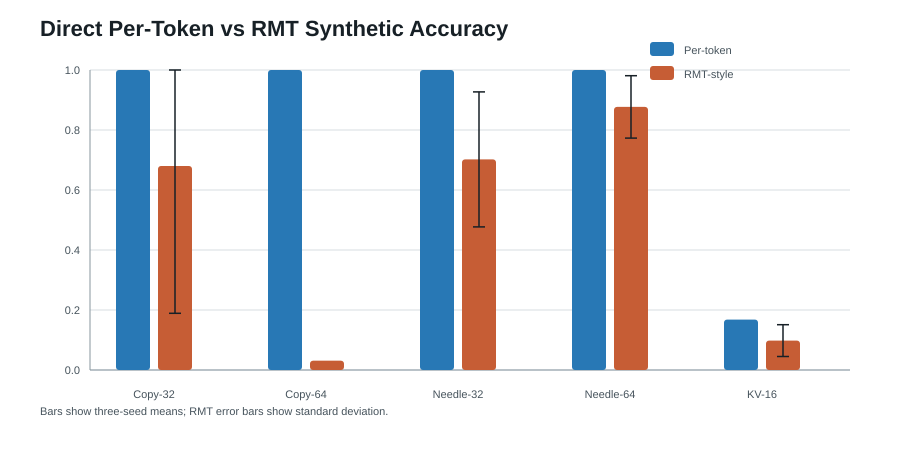
\includegraphics[width=0.85\linewidth]{figures/rmt_vs_per_token.pdf}
\caption{Mean accuracy with error bars (std.\ across three independent runs) for per-token
vs.\ RMT-style memory, corresponding to Table~\ref{tab:pertoken_vs_rmt}.
Per-token memory is at or near ceiling on every task; RMT-style memory is
competitive on needle retrieval but far more variable, especially on
copy-32.}
\label{fig:rmt_vs_per_token}
\end{figure}

\subsection{Token Salience and Retention}
\label{sec:salience-retention}

Per-token memory's advantage raises a mechanistic question: is every
token's memory slot actually needed, or does per-token memory contain
redundancy that a coarser allocation could also capture? For a trained
per-token model, we ablate each token's compressed key/value memory in
turn to rank slots by salience, then retain only the top-ranked fraction
at evaluation time (dropped slots are replaced with zero memory). Random
and uniform-stride retention at the same memory fraction serve as
same-budget controls. As with all synthetic results in
Section~\ref{sec:results}, accuracy here is teacher-forced
(Section~\ref{sec:synthetic-recall}); this experiment characterizes what
is accessible in memory under ablation, not robustness under free
generation.

\begin{table}[h]
\centering
\caption{Token retention at matched memory fractions: oracle salience
ranking vs.\ random and stride controls.}
\label{tab:retention}
\begin{tabular}{llrrr}
\toprule
Task & Method & Memory Kept & Accuracy & Loss \\
\midrule
Copy-32   & full          & 100\% & 1.000 & 2.019 \\
Copy-32   & oracle top-$k$ & 50\%  & 0.983 & 2.053 \\
Copy-32   & random top-$k$ & 50\%  & 0.509 & 5.351 \\
Copy-32   & stride top-$k$ & 50\%  & 0.492 & 4.639 \\
Copy-32   & oracle top-$k$ & 25\%  & 0.463 & 4.490 \\
Copy-32   & oracle top-$k$ & 10\%  & 0.191 & 5.897 \\
\addlinespace
KV-16     & full          & 100\% & 0.047 & 2.843 \\
KV-16     & oracle top-$k$ & 50\%  & 0.047 & 2.850 \\
KV-16     & random top-$k$ & 50\%  & 0.047 & 4.381 \\
KV-16     & stride top-$k$ & 50\%  & 0.047 & 4.781 \\
KV-16     & oracle top-$k$ & 10\%  & 0.047 & 3.353 \\
\addlinespace
Needle-64 & full          & 100\% & 0.062 & 3.931 \\
Needle-64 & oracle top-$k$ & 50\%  & 0.078 & 4.027 \\
Needle-64 & zero memory   & 0\%   & 0.016 & 4.339 \\
\bottomrule
\end{tabular}
\end{table}

\begin{figure}[h]
\centering
\includegraphics[width=0.75\linewidth]{figures/retention_copy32.pdf}
\caption{Copy-32 accuracy at matched 50\% memory budget: oracle
salience-based selection nearly matches the full-memory ceiling, while
random and stride selection at the identical budget collapse toward
chance.}
\label{fig:retention}
\end{figure}

Copy-32 gives the clearest result: oracle-selected top-50\% token memory
nearly matches full per-token accuracy (0.983 vs.\ 1.000), while random and
stride retention at the identical 50\% memory budget collapse to
near-chance (0.509 and 0.492). This is direct evidence that per-token
memory contains real redundancy -- not every token needs a dedicated slot
-- but that the useful slots are not interchangeable with an arbitrary
same-sized subset. KV-16 shows the same separation in loss (oracle 2.850
vs.\ random 4.381 and stride 4.781 at 50\% memory) but not in accuracy,
because the full-memory model's exact-match accuracy on this task is
already near floor (0.047) in this evaluation setup, leaving no headroom
for retention method to show up as an accuracy difference. Needle-64 is
not usable evidence here for the same reason: full-memory accuracy (0.062)
is too low for a retention comparison to be informative, since the base
model had not learned the task well enough to establish what
``near-full-memory'' performance looks like.

The safe reading is that per-token memory has meaningful redundancy at
this scale and budget -- roughly half the slots capture most of copy-32's
accessible information under oracle selection -- but this redundancy is
structured around specific salient tokens rather than being uniform, and
dense exact recall still degrades sharply once compression drops below
about 50\% of memory, even under the best-case oracle selection.

\subsection{RMT Changes the Recurrent-Memory Story}
\label{sec:rmt-recurrent-story}

The RMT-style baseline is much stronger than the custom recurrent updater
on long-gap needle retrieval (Table~\ref{tab:rmt_vs_recurrent}), after
correcting for a parameter-count confound: RMT's design includes an
unconditional learned initial-memory parameter that the custom recurrent
baseline did not originally have. Once the custom recurrent baseline was
given the same learned-initial-memory capacity, the needle-64 gap remained
essentially unchanged, confirming the RMT advantage is not an artifact of
that confound.

\begin{table}[h]
\centering
\caption{Custom recurrent vs.\ RMT-style memory on needle-64, after
parameter-count correction, three independent runs.}
\label{tab:rmt_vs_recurrent}
\begin{tabular}{llrrrrr}
\toprule
Task & Model & Run 1 & Run 2 & Run 3 & Mean & Std \\
\midrule
Needle-64 & Custom recurrent & 0.015 & 0.016 & 0.013 & 0.015 & 0.002 \\
Needle-64 & RMT-style        & 0.903 & 0.966 & 0.763 & 0.877 & 0.104 \\
\bottomrule
\end{tabular}
\end{table}

This result prevents the broad claim that all few-rich recurrent memory is
weak. Instead, the result is more precise: naive recurrent summarization is
weak for these tasks, while RMT-style memory tokens can support sparse
salient retrieval. However, RMT still does not beat per-token memory in the
direct comparison (Table~\ref{tab:pertoken_vs_rmt}), and does not improve
dense copy accuracy over custom recurrent at length 64 (both near 0.03).

\subsection{Associative Recurrent Memory: A Negative Result}
\label{sec:assoc-negative}

The associative branch tests whether explicit read/write addressing
(Section~\ref{sec:assoc-model}) and write-source normalization can
substantially narrow the gap to per-token memory. Full per-run tables
and diagnostics are reported in Appendix~A; the summary across three or
more independent runs is as follows:
\begin{itemize}[leftmargin=*]
  \item Write-normalized associative memory on needle-32 is highly
  variable across runs and, more specifically, \emph{bimodal}: two of four
  runs land near ceiling (0.591, 0.999) and two land near floor (0.029,
  0.019), with no clustering around an intermediate value.
  \item Raw associative memory at 2$\times$ memory budget on needle-64
  shows high run-to-run variance: the best of four runs achieves 0.227
  while the remaining three fall in the 0.015--0.018 range. The
  best run's read entropy of 6.238 is within 0.001 of $\ln(512)$, the
  theoretical maximum for uniform attention over 512 slots, indicating
  the elevated accuracy reflects broad averaging across slots rather than
  sharp content-addressed lookup.
  \item Associative memory did not solve dense copy at length 64 or random
  KV retrieval under any tested variant.
\end{itemize}
This branch remains useful as diagnostic evidence: simple structured
addressing is not sufficient to match many-small per-token memory under
these budgets, and Proposition~1 together with the collected diagnostics
(write entropy, slot usage, memory update norms) localizes the
contributing magnitude-instability issue to the write projection rather
than the gated recurrence itself.

% ===========================================================================
\section{Discussion}
% ===========================================================================

The results suggest a capacity-allocation effect. Dense exact recall
requires preserving many token identities at once. Per-token memory
allocates the budget directly across token-indexed states, so the model
has one storage location per recent token. Few-rich memory must compress
many items into fewer recurrent slots. Changing the update rule, adding
associative reads/writes, or using RMT-style memory tokens can change which
sparse retrieval problems are solvable, but these mechanisms do not remove
the dense-recall advantage of token-indexed storage in the current
experiments.

The RMT result is the most important nuance. It shows that the failure of
the custom recurrent model is not enough to condemn recurrent memory in
general. RMT-style memory tokens recover long-gap needle retrieval, which
is precisely the kind of sparse salient task recurrent memory should be
able to support. The direct per-token comparison then clarifies the
boundary: RMT is a much stronger few-rich baseline than naive pooling or
associative addressing, but many-small per-token memory remains stronger
overall for exact synthetic recall. A separate, low-slot-count shape sweep
(Section~\ref{sec:realdata-results}, Table~\ref{tab:shapesweep}) further shows that even within the
few-rich family, how the fixed budget is split between slot count and slot
dimension changes outcomes -- many-slot, narrow-dimension shapes
consistently matched or outperformed few-slot, wide-dimension shapes at
equal total budget. The long-context extension (Section~\ref{sec:longcontext})
shows that the many-small vs.\ few-rich gap for dense recall is not a
short-context artifact: at a fixed 32,768-float recurrent budget held
constant across the entire length 128--1024 range, the gap persists
8--16x beyond the original length-64 evidence.

% ===========================================================================
\section{Limitations}
% ===========================================================================

Our experiments are intentionally controlled and operate at substantially
smaller scale than contemporary production language models. The largest
model studied contains approximately 35M parameters, so the conclusions
should not be interpreted as establishing a universal scaling law for
memory architectures; a 100M-parameter or frontier-scale study is a
natural next step. The real-data tables in Section~\ref{sec:realdata-results} are drawn
from one or two training runs per configuration, as noted in
Table~\ref{tab:realdata}. The long-context probe in
Section~\ref{sec:longcontext} is complete for baseline, per-token, and
custom recurrent memory through copy length 512 and needle gap 1024, but
RMT-style memory is only evaluated through gap 128; extending RMT-style
evaluation to the same range is a natural next step, and none of the
long-context rows have yet been repeated across multiple training runs.

Synthetic recall is evaluated using teacher-forced target-token
prediction. This design isolates information accessibility in memory but
does not measure error accumulation during unrestricted autoregressive
generation.

Our recurrent comparisons cover several update mechanisms, including
pooled updates, associative read/write memory, and RMT-style memory
tokens, but do not exhaust the broader design space of recurrent or
state-space memory architectures. In particular, architectures such as
Mamba, TransformerFAM, and other learned-memory mechanisms differ
substantially enough that direct comparison would introduce additional
architectural confounds; we discuss them as context in
Section~\ref{sec:related-work} rather than as matched baselines.
Similarly, RMT-style memory has been evaluated on synthetic tasks in this
work but not yet on the 35M real-data language modeling runs.

Finally, the token-salience analysis in Section~\ref{sec:salience-retention}
uses an oracle post-hoc ranking and therefore demonstrates the existence
of redundancy rather than providing a deployable mechanism for selecting
which memories to retain. Learning such a selection policy is a natural
direction for future work.

This paper should therefore be read as a careful matched-budget study at a
bounded scale and context length, not as a universal law of memory
architectures.

% ===========================================================================
\section{Conclusion}
% ===========================================================================

Under matched persistent-memory budgets, per-token memory provides the
strongest performance among the methods tested here for language modeling
and for memory accessibility on exact-recall tasks. Few-rich recurrent
memory is not uniformly bad: RMT-style memory tokens are strong for
sparse long-gap single-fact retrieval. But in direct comparisons across
copy, needle, and random KV retrieval, per-token memory remains the most
reliable strategy for making the correct information accessible in
memory.

% ===========================================================================
\appendix
\section{Additional Results}
% ===========================================================================

\subsection{Associative Memory: Copy and Random-KV Probes}

Table~\ref{tab:assoc_copy} compares naive recurrent memory against explicit
associative read/write memory on the copy task, at the same \texttt{256x128}
persistent-memory shape. The associative model has more parameters, since
it adds explicit read/write projections (Section~\ref{sec:memory-budget}).

\begin{table}[h]
\centering
\caption{Naive recurrent vs.\ associative recurrent, copy task, matched
\texttt{256x128} memory shape.}
\label{tab:assoc_copy}
\begin{tabular}{lrr}
\toprule
Copy Length & Naive Recurrent & Assoc.\ Recurrent \\
\midrule
16 & 0.942 & 0.998 \\
32 & 0.046 & 0.064 \\
64 & 0.031 & 0.023 \\
\bottomrule
\end{tabular}
\end{table}

Associative memory improves short and medium copy length but does not solve
long exact copying. At length 64, the associative memory values become
unstable (delta norm 2141.6, value norm 2309.0 -- against naive recurrent's
1.6 and 1.6 at the same length), motivating the write-source normalization
tested next.

\begin{table}[h]
\centering
\caption{Raw vs.\ write-normalized associative memory, copy task.}
\label{tab:assoc_copy_writenorm}
\begin{tabular}{lrr}
\toprule
Copy Length & Assoc.\ Raw & Assoc.\ Write-Norm \\
\midrule
16 & 0.998 & 0.941 \\
32 & 0.064 & 0.053 \\
64 & 0.023 & 0.023 \\
\bottomrule
\end{tabular}
\end{table}

Write-source normalization controls the magnitude instability (token-out
norm at length 64 drops from an unstable regime to 732.8, and value norm to
24.0) but does not improve dense exact copying -- consistent with the copy
failure being a multi-item capacity problem rather than only a write-scale
problem.

Table~\ref{tab:assoc_copy2x} isolates the effect of doubling the few-rich
memory budget alone (\texttt{256x128} $\to$ \texttt{512x128}, raw
associative, no normalization).

\begin{table}[h]
\centering
\caption{Effect of doubling few-rich memory budget on copy-64.}
\label{tab:assoc_copy2x}
\begin{tabular}{llrrr}
\toprule
Model & Shape & Params & Mem Floats & Copy-64 \\
\midrule
Naive recurrent & \texttt{256x128} & 471{,}936 & 32{,}768 & 0.031 \\
Assoc.\ recurrent & \texttt{256x128} & 632{,}704 & 32{,}768 & 0.023 \\
Naive recurrent & \texttt{512x128} & 471{,}936 & 65{,}536 & 0.031 \\
Assoc.\ recurrent & \texttt{512x128} & 698{,}240 & 65{,}536 & 0.023 \\
\bottomrule
\end{tabular}
\end{table}

Doubling the budget does not improve copy-64 for either variant. Because
copy accuracy is measured over many copied tokens (195{,}000 predictions at
this length), this tie is not a coarse-evaluation artifact. The naive
recurrent write entropy at \texttt{512x128} is 0.693 -- within 0.001 of
$\ln(2)$ -- indicating the model writes to roughly two of the 512 available
slots regardless of how many exist, which is a more specific mechanism than
``more budget did not help.''

Table~\ref{tab:assoc_kv} reports the same naive-vs-associative comparison on
random key--value retrieval, at matched \texttt{256x128} shape.

\begin{table}[h]
\centering
\caption{Naive recurrent vs.\ associative recurrent, random KV retrieval,
matched \texttt{256x128} memory shape.}
\label{tab:assoc_kv}
\begin{tabular}{lrr}
\toprule
Pairs & Naive Recurrent & Assoc.\ Recurrent \\
\midrule
4  & 0.328 & 0.314 \\
8  & 0.234 & 0.222 \\
16 & 0.123 & 0.121 \\
\bottomrule
\end{tabular}
\end{table}

Associative memory is slightly worse than naive recurrent at every tested
pair count here, despite more parameters at the same memory budget.
Write-source normalization does not change this picture
(Table~\ref{tab:assoc_kv_writenorm}) -- it leaves 4 and 8 pairs unchanged
and is measurably worse at 16 pairs (0.121 $\to$ 0.107), indicating the
gap-32 needle improvement seen in Table~\ref{tab:assoc_needle32} is
task-specific rather than a general retrieval improvement.

\begin{table}[h]
\centering
\caption{Raw vs.\ write-normalized associative memory, random KV retrieval.}
\label{tab:assoc_kv_writenorm}
\begin{tabular}{lrr}
\toprule
Pairs & Assoc.\ Raw & Assoc.\ Write-Norm \\
\midrule
4  & 0.314 & 0.314 \\
8  & 0.222 & 0.222 \\
16 & 0.121 & 0.107 \\
\bottomrule
\end{tabular}
\end{table}

\subsection{Last-Token Recurrent Update}

Section~\ref{sec:custom-recurrent} lists mean pooling, cross-attention, and a last-token update as
the three tested naive-recurrent write mechanisms. Table~\ref{tab:lasttoken}
reports the last-token variant against cross-attention on both copy and
needle, at matched shape.

\begin{table}[h]
\centering
\caption{Cross-attention vs.\ last-token recurrent update.}
\label{tab:lasttoken}
\begin{tabular}{lrr}
\toprule
Task / Length & Cross-Attn Recurrent & Last-Token Recurrent \\
\midrule
Copy-16   & 0.942 & 0.942 \\
Copy-32   & 0.045 & 0.046 \\
Copy-64   & 0.030 & 0.031 \\
Needle-16 & 1.000 & 1.000 \\
Needle-32 & 0.016 & 0.016 \\
Needle-64 & 0.015 & 0.018 \\
\bottomrule
\end{tabular}
\end{table}

The last-token update does not fix the recurrent collapse either, indicating
the naive-recurrent failure is not specific to mean pooling or
cross-attention -- a third, structurally different update rule shows the
same pattern.

\subsection{Associative Memory: Additional Runs and Diagnostics}

Table~\ref{tab:assoc_needle32} reports results across repeated runs for
write-normalized associative memory on needle-32, showing the bimodal
pattern summarized in Section~\ref{sec:assoc-negative}.

\begin{table}[h]
\centering
\caption{Write-normalized associative memory, needle gap 32, four independent runs.}
\label{tab:assoc_needle32}
\begin{tabular}{lr}
\toprule
Run & Needle-32 Accuracy \\
\midrule
0 & 0.591 \\
1 & 0.029 \\
2 & 0.019 \\
3 & 0.999 \\
\bottomrule
\end{tabular}
\end{table}

Table~\ref{tab:assoc_needle64_2x} reports results across repeated runs for raw
associative memory at 2x memory budget on needle-64.

\begin{table}[h]
\centering
\caption{Raw associative memory, \texttt{512x128} shape (2x budget),
needle gap 64, four independent runs.}
\label{tab:assoc_needle64_2x}
\begin{tabular}{lr}
\toprule
Run & Needle-64 Accuracy \\
\midrule
0 & 0.227 \\
1 & 0.018 \\
2 & 0.017 \\
3 & 0.015 \\
\bottomrule
\end{tabular}
\end{table}

Diagnostics for the best-performing run in
Table~\ref{tab:assoc_needle64_2x} (naive recurrent shown for comparison):

\begin{table}[h]
\centering
\caption{Diagnostics at \texttt{512x128} shape, needle-64, first run.}
\begin{tabular}{lrrrrrr}
\toprule
Model & Read Entropy & Write Entropy & Delta Norm & Value Norm & Token Out Norm & Candidate Norm \\
\midrule
Naive recurrent & -- & 3.190 & 0.044 & 0.075 & -- & -- \\
Assoc.\ recurrent & 6.238 & 3.112 & 10.498 & 6.861 & 36.120 & 29.309 \\
\bottomrule
\end{tabular}
\end{table}

\noindent The assoc.\ recurrent read entropy of 6.238 is within 0.001 of
$\ln(512) \approx 6.2383$, the maximum possible entropy for a uniform
distribution over 512 slots. This indicates that the best-run improvement
in Table~\ref{tab:assoc_needle64_2x} reflects broad averaging across memory
slots rather than sharp, selective content-addressed retrieval -- the
intended associative-lookup behavior is not realized.

\begin{thebibliography}{99}

\bibitem[Bulatov et al.(2022)]{bulatov2022rmt}
Aydar Bulatov, Yuri Kuratov, and Mikhail Burtsev.
\newblock Recurrent Memory Transformer.
\newblock In \emph{Advances in Neural Information Processing Systems (NeurIPS)}, 2022.

\bibitem[Rodkin et al.(2024)]{rodkin2024armt}
Ivan Rodkin, Yuri Kuratov, Aydar Bulatov, and Mikhail Burtsev.
\newblock Associative Recurrent Memory Transformer.
\newblock \emph{arXiv preprint arXiv:2407.04841}, 2024.

\bibitem[Hwang et al.(2024)]{hwang2024transformerfam}
Dongseong Hwang, Weiran Wang, Zhuoyuan Huo, Khe Chai Sim, and Pedro Moreno Mengibar.
\newblock TransformerFAM: Feedback attention is working memory.
\newblock \emph{arXiv preprint arXiv:2404.09173}, 2024.

\bibitem[Dai et al.(2019)]{dai2019transformerxl}
Zihang Dai, Zhilin Yang, Yiming Yang, Jaime Carbonell, Quoc V. Le, and Ruslan Salakhutdinov.
\newblock Transformer-XL: Attentive Language Models Beyond a Fixed-Length Context.
\newblock In \emph{Proceedings of the 57th Annual Meeting of the Association for Computational Linguistics (ACL)}, 2019.

\bibitem[Rae et al.(2020)]{rae2020compressive}
Jack W. Rae, Anna Potapenko, Siddhant M. Jayakumar, and Timothy P. Lillicrap.
\newblock Compressive Transformers for Long-Range Sequence Modelling.
\newblock In \emph{International Conference on Learning Representations (ICLR)}, 2020.

\bibitem[Wu et al.(2022)]{wu2022memorizing}
Yuhuai Wu, Markus N. Rabe, DeLesley Hutchins, and Christian Szegedy.
\newblock Memorizing Transformers.
\newblock In \emph{International Conference on Learning Representations (ICLR)}, 2022.

\bibitem[Munkhdalai et al.(2024)]{munkhdalai2024infini}
Tsendsuren Munkhdalai, Manaal Faruqui, and Siddharth Gopal.
\newblock Leave No Context Behind: Efficient Infinite Context Transformers with Infini-attention.
\newblock \emph{arXiv preprint arXiv:2404.07143}, 2024.

\bibitem[Chen et al.(2024)]{chen2024melodi}
Yinpeng Chen, DeLesley Hutchins, Aren Jansen, Andrey Zhmoginov, David Racz, and Jesper Andersen.
\newblock MELODI: Exploring Memory Compression for Long Contexts.
\newblock \emph{arXiv preprint arXiv:2410.03156}, 2024.

\bibitem[Goldstein et al.(2026)]{goldstein2026kvm}
Daniel Goldstein, Navneel Singhal, and Eugene Cheah.
\newblock Key-Value Means: Transformers with Expandable Block-Recurrent Compressed Memory.
\newblock \emph{arXiv preprint arXiv:2605.09877}, 2026.

\bibitem[Xiao et al.(2023)]{xiao2023streaming}
Guangxuan Xiao, Yuandong Tian, Beidi Chen, Song Han, and Mike Lewis.
\newblock Efficient Streaming Language Models with Attention Sinks.
\newblock \emph{arXiv preprint arXiv:2309.17453}, 2023.

\bibitem[Gu and Dao(2023)]{gu2023mamba}
Albert Gu and Tri Dao.
\newblock Mamba: Linear-Time Sequence Modeling with Selective State Spaces.
\newblock \emph{arXiv preprint arXiv:2312.00752}, 2023.

\bibitem[Eldan and Li(2023)]{eldan2023tinystories}
Ronen Eldan and Yuanzhi Li.
\newblock TinyStories: How Small Can Language Models Be and Still Speak Coherent English?
\newblock \emph{arXiv preprint arXiv:2305.07759}, 2023.

\bibitem[Merity et al.(2017)]{merity2017wikitext}
Stephen Merity, Caiming Xiong, James Bradbury, and Richard Socher.
\newblock Pointer Sentinel Mixture Models.
\newblock In \emph{International Conference on Learning Representations (ICLR)}, 2017.

\bibitem[Hutchins et al.(2022)]{hutchins2022blockrecurrent}
DeLesley Hutchins, Imanol Schlag, Yuhuai Wu, Ethan Dyer, and Behnam Neyshabur.
\newblock Block-Recurrent Transformers.
\newblock In \emph{Advances in Neural Information Processing Systems (NeurIPS)}, 2022.

\bibitem[Wang et al.(2023)]{wang2023longmem}
Weizhi Wang, Li Dong, Hao Cheng, Xiaodong Liu, Xifeng Yan, Jianfeng Gao, and Furu Wei.
\newblock Augmenting Language Models with Long-Term Memory.
\newblock In \emph{Advances in Neural Information Processing Systems (NeurIPS)}, 2023.

\bibitem[Behrouz et al.(2025)]{behrouz2025titans}
Ali Behrouz, Peilin Zhong, and Vahab Mirrokni.
\newblock Titans: Learning to Memorize at Test Time.
\newblock \emph{arXiv preprint arXiv:2501.00663}, 2025.

\bibitem[Ainslie et al.(2023)]{ainslie2023gqa}
Joshua Ainslie, James Lee-Thorp, Michiel de Jong, Yury Zemlyanskiy, Federico Lebrón, and Sumit Sanghai.
\newblock GQA: Training Generalized Multi-Query Transformer Models from Multi-Head Checkpoints.
\newblock In \emph{Proceedings of the 2023 Conference on Empirical Methods in Natural Language Processing (EMNLP)}, 2023.

\bibitem[DeepSeek-AI(2024)]{deepseek2024v2}
DeepSeek-AI.
\newblock DeepSeek-V2: A Strong, Economical, and Efficient Mixture-of-Experts Language Model.
\newblock \emph{arXiv preprint arXiv:2405.04434}, 2024.

\bibitem[Nawrot et al.(2024)]{nawrot2024dmc}
Piotr Nawrot, Adrian Łańcucki, Marcin Chochowski, David Tarjan, and Edoardo M. Ponti.
\newblock Dynamic Memory Compression: Retrofitting LLMs for Accelerated Inference.
\newblock In \emph{International Conference on Machine Learning (ICML)}, 2024.

\bibitem[Liu et al.(2024a)]{liu2024kivi}
Zirui Liu, Jiayi Yuan, Hongye Jin, Shaochen Zhong, Zhaozhuo Xu, Vladimir Braverman, Beidi Chen, and Xia Hu.
\newblock KIVI: A Tuning-Free Asymmetric 2bit Quantization for KV Cache.
\newblock \emph{arXiv preprint arXiv:2402.02750}, 2024.

\bibitem[Zhang et al.(2023)]{zhang2023h2o}
Zhenyu Zhang, Ying Sheng, Tianyi Zhou, Tianlong Chen, Lianmin Zheng, Ruisi Cai, Zhao Song, Yuandong Tian, Christopher Ré, Clark Barrett, Zhangyang Wang, and Beidi Chen.
\newblock H$_2$O: Heavy-Hitter Oracle for Efficient Generative Inference of Large Language Models.
\newblock In \emph{Advances in Neural Information Processing Systems (NeurIPS)}, 2023.

\bibitem[Liu et al.(2023)]{liu2023scissorhands}
Zichang Liu, Aditya Desai, Fangshuo Liao, Weitao Wang, Victor Xie, Zhaozhuo Xu, Anastasios Kyrillidis, and Anshumali Shrivastava.
\newblock Scissorhands: Exploiting the Persistence of Importance Hypothesis for LLM KV Cache Compression at Test Time.
\newblock In \emph{Advances in Neural Information Processing Systems (NeurIPS)}, 2023.

\bibitem[Li et al.(2024)]{li2024snapkv}
Yuhong Li, Yingbing Huang, Bowen Yang, Bharat Venkitesh, Acyr Locatelli, Hanchen Ye, Tianle Cai, Patrick Lewis, and Deming Chen.
\newblock SnapKV: LLM Knows What You are Looking for Before Generation.
\newblock \emph{arXiv preprint arXiv:2404.14469}, 2024.

\bibitem[Cai et al.(2025)]{cai2025pyramidkv}
Zefan Cai, Yichi Zhang, Bofei Gao, Yuliang Liu, Yucheng Li, Tianyu Liu, Keming Lu, Wayne Xiong, Yue Dong, Junjie Hu, et al.
\newblock PyramidKV: Dynamic KV Cache Compression based on Pyramidal Information Funneling.
\newblock \emph{arXiv preprint arXiv:2406.02069}, 2025.

\bibitem[Tang et al.(2024)]{tang2024quest}
Jiaming Tang, Yilong Zhao, Kan Zhu, Guangxuan Xiao, Baris Kasikci, and Song Han.
\newblock Quest: Query-Aware Sparsity for Efficient Long-Context LLM Inference.
\newblock In \emph{International Conference on Machine Learning (ICML)}, 2024.

\bibitem[Xiao et al.(2025)]{xiao2025duoattention}
Guangxuan Xiao, Jiaming Tang, Jingwei Zuo, Junxian Guo, Shang Yang, Haotian Tang, Yao Fu, and Song Han.
\newblock DuoAttention: Efficient Long-Context LLM Inference with Retrieval and Streaming Heads.
\newblock In \emph{International Conference on Learning Representations (ICLR)}, 2025.

\bibitem[Sun et al.(2023)]{sun2023retnet}
Yutao Sun, Li Dong, Shaohan Huang, Shuming Ma, Yuqing Xia, Jilong Xue, Jianyong Wang, and Furu Wei.
\newblock Retentive Network: A Successor to Transformer for Large Language Models.
\newblock \emph{arXiv preprint arXiv:2307.08621}, 2023.

\bibitem[Peng et al.(2023)]{peng2023rwkv}
Bo Peng, Eric Alcaide, Quentin Anthony, Alon Albalak, Samuel Arcadinho, Huanqi Cao, Xin Cheng, Michael Chung, Matteo Grella, et al.
\newblock RWKV: Reinventing RNNs for the Transformer Era.
\newblock \emph{arXiv preprint arXiv:2305.13048}, 2023.

\bibitem[De et al.(2024)]{de2024griffin}
Soham De, Samuel L. Smith, Anushan Fernando, Aleksandar Botev, George Cristian-Muraru, Albert Gu, Ruba Haroun, Leonard Berrada, Yutian Chen, Srivatsan Srinivasan, Guillaume Desjardins, Arnaud Doucet, David Budden, Yee Whye Teh, Razvan Pascanu, Nando De Freitas, and Caglar Gulcehre.
\newblock Griffin: Mixing Gated Linear Recurrences with Local Attention for Efficient Language Models.
\newblock \emph{arXiv preprint arXiv:2402.19427}, 2024.

\end{thebibliography}

\end{document}
